\documentclass[11pt,a4paper]{article}

% --- Page Geometry (Standard Academic A4 Dimensions) ---
\setlength{\paperwidth}{210mm}
\setlength{\paperheight}{297mm}
\setlength{\textwidth}{166mm}
\setlength{\textheight}{244mm}
\setlength{\oddsidemargin}{-3.0mm}
\setlength{\evensidemargin}{-3.0mm}
\setlength{\topmargin}{-10.0mm}
\setlength{\headheight}{14pt}
\setlength{\headsep}{16pt}
\setlength{\footskip}{24pt}

% --- Typography & Font Configuration ---
\renewcommand{\rmdefault}{ptm} % Times Roman NFSS font
\usepackage{amsmath,amssymb}
\usepackage{graphicx}
\usepackage{xcolor}
\usepackage{array}
\usepackage{tabularx}
\usepackage{url}

% Custom Color Definitions
\definecolor{nexaNavy}{RGB}{30,58,138}    % #1e3a8a (Primary Headings)
\definecolor{nexaSlate}{RGB}{30,41,59}    % #1e293b (Secondary Headings)
\definecolor{nexaDark}{RGB}{15,23,42}     % #0f172a (Body Text)
\definecolor{nexaMuted}{RGB}{71,85,105}   % #475569 (Captions & Headers)
\definecolor{nexaBlue}{RGB}{37,99,235}    % #2563eb (Links & Highlights)

% Hyperlink configuration using url and xcolor
\newcommand{\projectlink}[2]{\textcolor{nexaBlue}{\underline{#2}}\footnote{\url{#1}}}
\newcommand{\codetext}[1]{\texttt{\small #1}}

% Paragraph & Section Spacing
\setlength{\parindent}{0pt}
\setlength{\parskip}{2.8pt plus 0.4pt minus 0.4pt}
\setcounter{tocdepth}{1} % Match original report TOC structure (Sections only)

% Custom Section Header Styling without extra packages
\makeatletter
\renewcommand\section{\@startsection {section}{1}{\z@}%
  {-9pt \@plus -2pt \@minus -.5pt}%
  {3pt \@plus .5pt}%
  {\normalfont\large\bfseries\color{nexaNavy}}}
\renewcommand\subsection{\@startsection{subsection}{2}{\z@}%
  {-7pt \@plus -1.5pt \@minus -.5pt}%
  {2pt \@plus .5pt}%
  {\normalfont\normalsize\bfseries\color{nexaSlate}}}
\renewcommand\subsubsection{\@startsection{subsubsection}{3}{\z@}%
  {-5pt \@plus -1pt \@minus -.5pt}%
  {1.5pt \@plus .5pt}%
  {\normalfont\small\bfseries\itshape\color{nexaSlate}}}
\makeatother

% Running Headers & Footers
\makeatletter
\def\ps@nexaReport{%
  \def\@oddhead{\small\itshape\color{nexaMuted}NexaVault --- Departmental Academic Project Evaluation Platform\hfill\thepage}%
  \def\@evenhead{\small\itshape\color{nexaMuted}\thepage\hfill NexaVault --- Departmental Academic Project Evaluation Platform}%
  \def\@oddfoot{\footnotesize\color{nexaMuted}Institutional Course: 23AID204 Advanced DSA\hfill School of Artificial Intelligence, Amrita Vishwa Vidyapeetham}%
  \def\@evenfoot{\footnotesize\color{nexaMuted}School of Artificial Intelligence, Amrita Vishwa Vidyapeetham\hfill Institutional Course: 23AID204 Advanced DSA}%
}
\def\ps@nexaTOC{%
  \def\@oddhead{}%
  \def\@evenhead{}%
  \def\@oddfoot{\hfill\small\thepage\hfill}%
  \def\@evenfoot{\hfill\small\thepage\hfill}%
}
\makeatother

\begin{document}

% ==============================================================================
% COVER PAGE (PRESERVED 100% IDENTICAL TO INSTITUTIONAL SPECIFICATION)
% ==============================================================================
\begin{titlepage}
\thispagestyle{empty}
\centering
\vspace*{0.2cm}

{\Large\bfseries AMRITA VISHWA VIDYAPEETHAM}\par
\vspace{0.6cm}


\includegraphics[width=4.8in,keepaspectratio]{figures/amrita_logo.png}\par
\vspace{0.6cm}

{\large\bfseries SCHOOL OF ARTIFICIAL INTELLIGENCE \textbar\ COIMBATORE}\par
\vspace{1.2cm}

{\huge\bfseries PROJECT REPORT}\par
\vspace{0.4cm}
{\huge\bfseries\color{nexaNavy} NexaVault}\par
\vspace{0.8cm}

{\large\bfseries Done by}\par
\vspace{0.3cm}
{\normalsize
\textbf{CB.AI.U4AID25008} -- GURUCHARAN \quad
\textbf{CB.AI.U4AID25049} -- SHARVESH \par\vspace{0.2cm}
\textbf{CB.AI.U4AID25062} -- BHAVESH JAYAN \quad
\textbf{CB.AI.U4AID25064} -- HASHWIN\par}
\vspace{1.2cm}

{\large\bfseries Institutional Course}\par
\vspace{0.2cm}
{\large\bfseries 23AID204 \textbar\ Advanced Data Structures \& Algorithm Analysis}\par
\vspace{1.0cm}

{\large\bfseries Faculty In-Charge}\par
\vspace{0.2cm}
{\large\bfseries Dr. Ardra P. S.}\par
\vspace{1.2cm}

{\large\bfseries SCHOOL OF ARTIFICIAL INTELLIGENCE}\par
\vspace*{0.4cm}
\end{titlepage}

\clearpage

% ==============================================================================
% TABLE OF CONTENTS (PAGE 2)
% ==============================================================================
\pagestyle{nexaTOC}
\setcounter{page}{2}

\begin{center}
  {\Large\bfseries\color{nexaNavy} TABLE OF CONTENTS}\par
\end{center}
\vspace{0.2cm}

\renewcommand{\contentsname}{}
\vspace{-1.0cm}
{
  \makeatletter
  \renewcommand{\@pnumwidth}{1.8em}
  \renewcommand{\@tocrmarg}{2.5em}
  \makeatother
  \tableofcontents
}

\clearpage

% ==============================================================================
% REPORT BODY (PAGES 3 - 12)
% ==============================================================================
\pagestyle{nexaReport}
\setcounter{page}{3}

\section{Abstract}
\textbf{NexaVault} is an enterprise-grade academic collaborative workspace and continuous project evaluation platform engineered to resolve the operational bottlenecks of departmental computer science laboratory courses and capstone milestones. Developed for university project courses such as 23AID204 (Advanced Data Structures and Algorithm Analysis), the platform unifies self-service student group formation, workspace curriculum management, milestone deliverable submissions, faculty review queues with row-level concurrency locking, individual student rubric evaluations, dynamic multi-round results aggregation, and an automated 24-hour expiring notice board.

Built on a decoupled full-stack architecture comprising a React 18 single-page application (SPA), a high-throughput Python FastAPI REST backend, and a cloud-managed PostgreSQL 16 database hosted on Neon Serverless, NexaVault enforces strict transactional data integrity. Key engineering achievements include an immutable deliverable versioning pipeline that permanently captures a JSONB group-roster snapshot at submit time, PostgreSQL \texttt{SELECT ... FOR UPDATE} row-level locking that eliminates dual-grader collisions among faculty evaluators, and a thread-safe in-memory Least-Recently-Used (LRU) cache with an inverted tag index yielding an empirical 43-fold latency reduction ($35\,\text{ms} \to 0.8\,\text{ms}$) on cached workspace queries. Comprehensive verification confirms 100\% passing across all 44 automated backend test suites and an 8.64-second production build, demonstrating a resilient and transparent academic evaluation infrastructure.

\section{Introduction}
In modern computing curricula, collaborative laboratory projects and continuous multi-stage evaluations represent vital components of student assessment. In rigorous courses such as 23AID204, dozens of student teams design, implement, and present complex software implementations across multiple milestone reviews throughout the semester. However, administering these courses across academic departments routinely encounters severe logistical challenges when relying on fragmented, ad-hoc combinations of instant messaging, spreadsheets, external Git repositories, and generic learning management systems (LMS) such as Google Classroom or Moodle.

Generic LMS platforms are fundamentally assignment-centric rather than project-centric. They fail to support self-organized team formation with cryptographic join codes, lack support for versioned deliverable submissions linked to source control commits, and assign single aggregate grades to entire groups rather than evaluating individual contributions. Furthermore, when multiple faculty instructors and teaching assistants simultaneously assess laboratory queues, uncoordinated tools lead to evaluation collisions, conflicting feedback, and unrecorded grade alterations. NexaVault was architected from first principles to overcome these limitations through an integrated, concurrency-safe, role-isolated academic workspace.

\section{Problem Statement and Project Objectives}
\subsection{Problem Statement}
Academic project administration across computing departments suffers from five chronic systemic vulnerabilities:
\begin{enumerate}
  \item \textbf{Tool Fragmentation:} Student team rosters, milestone deliverables, Git repositories, faculty notices, and grading marksheets are scattered across disparate tools, resulting in data loss and heavy administrative overhead.
  \item \textbf{Evaluation Inconsistencies:} Standard platforms assign a single collective mark to an entire group, failing to distinguish individual student contributions and causing friction during grading appeals.
  \item \textbf{Grading Concurrency Collisions:} Multiple evaluators assessing submissions simultaneously lack centralized submission locking, leading to double-grading or overwritten rubric scores.
  \item \textbf{Information Perishability:} Critical laboratory announcements and deadline notices are buried under conversational chat threads without automated lifecycle expiration.
  \item \textbf{Audit Invisibility:} Grade revisions, administrative privilege grants, and resubmissions occur without immutable audit logging, compromising departmental accreditation compliance.
\end{enumerate}

\subsection{Project Objectives}
To address these vulnerabilities, NexaVault was implemented to fulfill the following objectives:
\begin{itemize}
  \item \textbf{Role-Based Access Control:} Implement secure, stateless JWT authentication with strict role isolation between Student, Faculty, and Admin accounts.
  \item \textbf{Self-Service Team Formation:} Enable students to form persistent collaborative groups via unique 6-character cryptographic join codes and decouple teams from workspaces via an Enrollment model.
  \item \textbf{Immutable Deliverable Versioning:} Support multi-round milestone submissions and freeze group membership rosters in JSONB at the exact second of submission.
  \item \textbf{Concurrency-Safe Review Queues:} Implement PostgreSQL \texttt{SELECT ... FOR UPDATE} row-level locking to guarantee mutually exclusive submission claiming across faculty reviewers.
  \item \textbf{Granular Rubric Evaluation:} Support multi-criteria rubric scoring and individual qualitative feedback per student, aggregated into dynamic universal CSV marksheets.
  \item \textbf{Automated Information Lifecycle:} Provide a faculty notice board with image validation and database-enforced 24-hour expiration queries with automated disk cleanup.
\end{itemize}

\section{Existing System and Proposed Solution}
\subsection{Limitations of the Existing System}
Conventional project evaluation relies heavily on generic commercial learning management systems supplemented by spreadsheets. While functional for homework collection, these platforms fail in collaborative software project workflows: they lack self-service team formation with join codes, do not capture versioned deliverable history linked to Git commits, cannot prevent two evaluators from grading the same submission concurrently, and provide static mark exports that fail to scale dynamically with multi-round weighted rubrics.

\subsection{The NexaVault Proposed Solution}
NexaVault resolves these deficiencies by introducing an integrated, domain-specific continuous evaluation platform. The system unifies team formation, workspace curriculum management, versioned deliverables, concurrency-controlled review queues, individual rubric scoring, and dynamic UTF-8 BOM CSV reporting within a single secure environment. Table~\ref{tab:comparison} contrasts traditional approaches with the NexaVault platform.

\begin{table}[htbp]
\centering
\small
\caption{Feature Comparison: Traditional Systems vs. NexaVault Platform}
\label{tab:comparison}
\vspace{0.15cm}
\begin{tabularx}{\textwidth}{|l|X|X|}
\hline\hline
\textbf{Functional Dimension} & \textbf{Traditional Systems (Generic LMS / Spreadsheets)} & \textbf{NexaVault Architecture} \\
\hline\hline
\textbf{Team Formation} & Manual spreadsheet entry or administrative CSV import & Self-service group creation with cryptographic join codes \\
\hline
\textbf{Roster Integrity} & Member shifts silently alter historical submissions & Immutable JSONB roster snapshots frozen at submit time \\
\hline
\textbf{Review Concurrency} & No locking; simultaneous evaluators overwrite scores & PostgreSQL \texttt{FOR UPDATE} row locks prevent collisions \\
\hline
\textbf{Grading Granularity} & Single aggregate score assigned to the collective group & Individual student rubric criteria marks and feedback \\
\hline
\textbf{Review Configuration} & Rigid, predefined assignment deadlines & Dynamic review rounds with weights, rubrics, and deadlines \\
\hline
\textbf{Marksheet Export} & Manual copy-paste or static spreadsheet dumps & Dynamic universal UTF-8 BOM CSV grouped by team \\
\hline
\textbf{Notice Lifecycle} & Permanent clutter or lost in messaging channels & Query-level 24-hour expiration with media disk cleanup \\
\hline\hline
\end{tabularx}
\end{table}

\section{System Requirements and Technology Stack}
\subsection{Software Requirements}
\begin{itemize}
  \item \textbf{Client Environment:} Cross-platform web browsers (Chrome $\ge$120, Firefox $\ge$120, Safari $\ge$17, Edge $\ge$120).
  \item \textbf{Backend Runtime:} Python 3.10+ running the FastAPI asynchronous framework on a Uvicorn ASGI server.
  \item \textbf{Database System:} PostgreSQL 16 hosted on Neon Managed Serverless PostgreSQL with SSL.
  \item \textbf{Containerization \& Proxy:} Docker Compose and Nginx reverse proxy for static assets and API routing.
\end{itemize}

\subsection{Verified Technology Stack}
\begin{itemize}
  \item \textbf{Frontend:} React 18.3.1 SPA scaffolded with Vite 6.0.7 for rapid HMR and optimized production compilation \cite{react2024, vite2024}. Styled using Tailwind CSS 3.4.17 with PostCSS. UI icons provided by Lucide React. Authentication state managed via React Context API (\texttt{AuthContext}) with in-memory keep-alive tab state caching.
  \item \textbf{Backend:} FastAPI ($\ge$0.110.0) running on Uvicorn ASGI server \cite{fastapi2024}. Request/response schema validation and environment management powered by Pydantic v2. Synchronous relational persistence handled by SQLAlchemy 2.0 ORM with connection pooling.
  \item \textbf{Persistence \& Migrations:} PostgreSQL 16 hosted on Neon Serverless Cloud Database with TLS encryption \cite{postgresql2023}. Schema versioning and zero-downtime structural evolutions managed via Alembic ($\ge$1.13.0).
  \item \textbf{Security \& Utilities:} Direct bcrypt ($\ge$4.1.2) password hashing with explicit 72-byte truncation \cite{provos1999bcrypt}. PyJWT ($\ge$2.8.0) HMAC-SHA256 stateless tokens with 24-hour expiration \cite{rfc7519jwt}. Pillow ($\ge$10.0.0) for media validation, and HTTPX ($\ge$0.27.0) for asynchronous GitHub REST API repository synchronization.
\end{itemize}

\subsection{Architectural Rationale}
FastAPI was selected over Django and Flask due to its high-throughput asynchronous execution model, automatic OpenAPI documentation, and native Pydantic v2 validation. PostgreSQL 16 on Neon Serverless was chosen over document databases (such as MongoDB) because academic evaluation strictly mandates ACID guarantees, relational foreign keys, and transactional row-level locks during grading claims. The React 18 SPA delivers immediate client-side responsiveness without page reloads.

\section{System Architecture and Design}
\subsection{System Architecture Overview}
NexaVault implements a modular three-tier architecture separating presentation, business logic, and relational persistence. The client-side single-page application communicates with the backend exclusively via authenticated RESTful JSON APIs over TLS. The architecture is illustrated in Figure~\ref{fig:architecture}.

\begin{figure}[htbp]
  \centering
  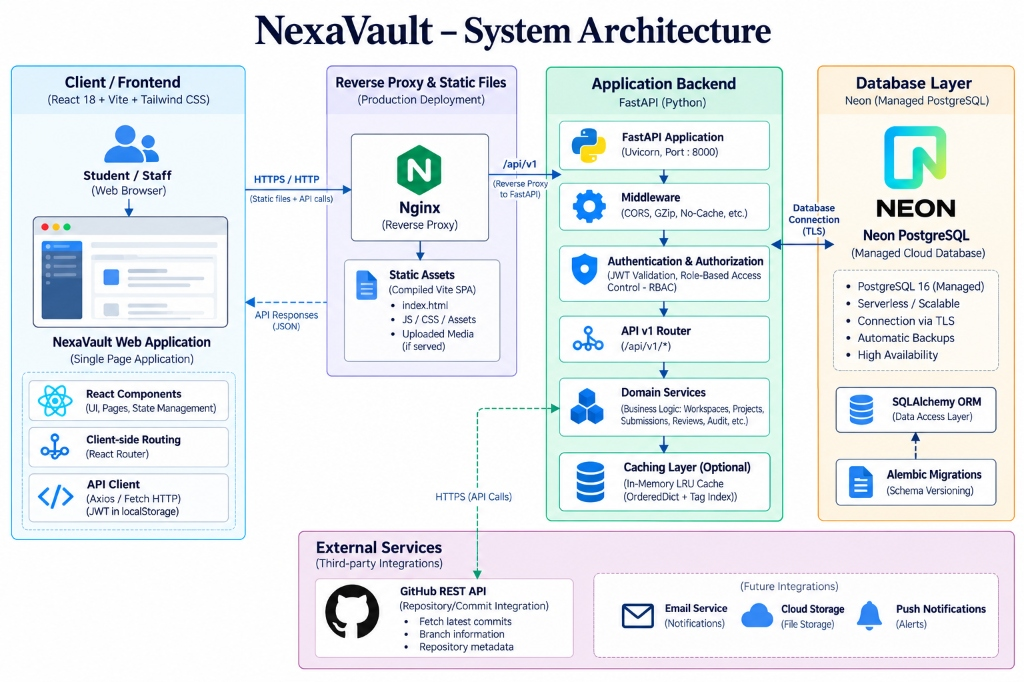
\includegraphics[width=0.96\textwidth,keepaspectratio]{figures/system_architecture.jpg}
  \caption{NexaVault Three-Tier System Architecture and Infrastructure Pipeline}
  \label{fig:architecture}
\end{figure}

\subsection{Architectural Components}
\begin{enumerate}
  \item \textbf{Client / Frontend Tier:} React 18 single-page application styled with Tailwind CSS. Role-based view routing renders dedicated Student and Staff interfaces while persisting stateless JWT tokens in \texttt{localStorage}.
  \item \textbf{Reverse Proxy \& Static Gateway:} Nginx reverse proxy serving compiled static assets (\texttt{index.html}, CSS, JavaScript) and proxying all \texttt{/api/v1/*} API traffic to the FastAPI application backend.
  \item \textbf{Application Backend:} FastAPI on Uvicorn (Port 8000) orchestrating CORS middleware, JWT validation, role-based dependency injection guards (\texttt{deps.py}), domain services, and an in-memory LRU cache.
  \item \textbf{Database Persistence Layer:} Neon Serverless PostgreSQL 16 communicating through SQLAlchemy 2.0 ORM with connection pooling and Alembic schema versioning migrations.
  \item \textbf{External Integrations:} Asynchronous communication with the GitHub REST API via HTTPX to retrieve repository branches, metadata, and commit hashes for deliverable submissions.
\end{enumerate}

\subsection{Core Relational Data Model}
The core data architecture decouples student groups from academic workspaces through an intermediate \texttt{Enrollment} entity. A \texttt{Group} represents a persistent collaborative team of students identified by a cryptographic join code. A \texttt{Workspace} represents an academic offering managed by faculty. An \texttt{Enrollment} establishes the formal participation of a group within a specific workspace, and a \texttt{Project} belongs strictly to an enrollment. This design allows student teams to persist across multiple academic terms or workspaces while maintaining independent project contexts, submissions, and evaluation histories.

\subsection{Request and Data Flow}
Every incoming client request follows a deterministic lifecycle: (1) TLS termination and CORS validation, (2) JWT Bearer token extraction and cryptographic signature verification, (3) Role-based dependency injection in FastAPI (\texttt{deps.require\_staff} or \texttt{deps.get\_current\_user}), (4) Cache lookup in the \texttt{InMemoryCache}, returning cached payloads immediately on hit, (5) Business logic execution within an isolated SQLAlchemy database session, (6) Automatic commit or rollback on error, (7) Targeted cache invalidation upon data mutation, and (8) Pydantic response serialization.

\section{Database Design and API Architecture}
\subsection{Normalized Relational Schema}
The NexaVault database comprises 16 core SQLAlchemy models structured in Third Normal Form (3NF) to eliminate data redundancy while enforcing relational integrity constraints. Schema changes are systematically tracked through Alembic migration scripts. Table~\ref{tab:database_models} summarizes the primary relational entities.

\begin{table}[htbp]
\centering
\small
\caption{Core Relational Database Entities, Primary Keys and Relational Constraints}
\label{tab:database_models}
\vspace{0.15cm}
\begin{tabularx}{\textwidth}{|l|l|X|}
\hline\hline
\textbf{Database Table} & \textbf{Primary \& Foreign Keys} & \textbf{Constraints \& Functional Purpose} \\
\hline\hline
\texttt{users} & PK: \texttt{id} (UUID) & Unique email index; bcrypt hash; role check (\texttt{student}, \texttt{staff}) \\
\hline
\texttt{workspaces} & PK: \texttt{id}, FK: \texttt{created\_by\_id} & Unique join code index; soft-archive flag; faculty association \\
\hline
\texttt{groups} & PK: \texttt{id}, FK: \texttt{leader\_id} & Unique team join code; foreign key to team creator user \\
\hline
\texttt{enrollments} & PK: \texttt{id}, FK: \texttt{group\_id}, \texttt{workspace\_id} & \texttt{UniqueConstraint(group\_id, workspace\_id)}; links teams to courses \\
\hline
\texttt{projects} & PK: \texttt{id}, FK: \texttt{enrollment\_id} & 1:1 with enrollment; tracks GitHub repository, live URL, tech stack \\
\hline
\texttt{review\_rounds} & PK: \texttt{id}, FK: \texttt{workspace\_id} & Round order, max score, percentage weight, rubrics, deadline \\
\hline
\texttt{submission\_versions} & PK: \texttt{id}, FK: \texttt{submission\_id}, \texttt{claimed\_by\_id} & Freezes \texttt{roster\_snapshot} (JSONB); \texttt{FOR UPDATE} row locking \\
\hline
\texttt{individual\_review\_scores} & PK: \texttt{id}, FK: \texttt{version\_id}, \texttt{student\_id} & Rubric criteria marks (JSONB), total score, qualitative feedback \\
\hline\hline
\end{tabularx}
\end{table}

\subsection{Transaction Management and Concurrency Row-Level Locking}
Database transactions are managed using SQLAlchemy scoped sessions with connection pooling. To eliminate grading collisions where two faculty evaluators simultaneously open and evaluate the same submission, NexaVault enforces row-level locking via PostgreSQL's \texttt{SELECT ... FOR UPDATE} syntax. In \texttt{app/api/v1/endpoints/reviews.py}, when an evaluator requests the \texttt{/claim} endpoint, the transaction locks the targeted \texttt{submission\_versions} record. Any concurrent claim request from another faculty member detects the existing lock, verifies that \texttt{claimed\_by\_id} is already assigned, and is rejected with an HTTP 400 conflict response.

\section{Implementation of Student and Staff Modules}
\subsection{Student Module Workflows}
The student module facilitates self-service team organization and transparent project execution. Students register accounts and either create a collaborative group or join an existing group using a 6-character cryptographic join code. Once grouped, teams enroll in active workspaces and register their project details, including title, abstract, tech stack tags, and GitHub repository URL. For each configured review round, students submit deliverable URLs, documentation links, or Git commit hashes. At the exact second of submission, the backend serializes the current group members into an immutable \texttt{roster\_snapshot} (JSONB), ensuring that subsequent team roster changes cannot alter past submission attribution. Students access a dedicated Results View displaying their individual rubric scores, weighted totals, and personalized faculty feedback. Figure~\ref{fig:student_module} shows the student interface.

\begin{figure}[htbp]
  \centering
  \begin{minipage}{0.49\textwidth}
    \centering
    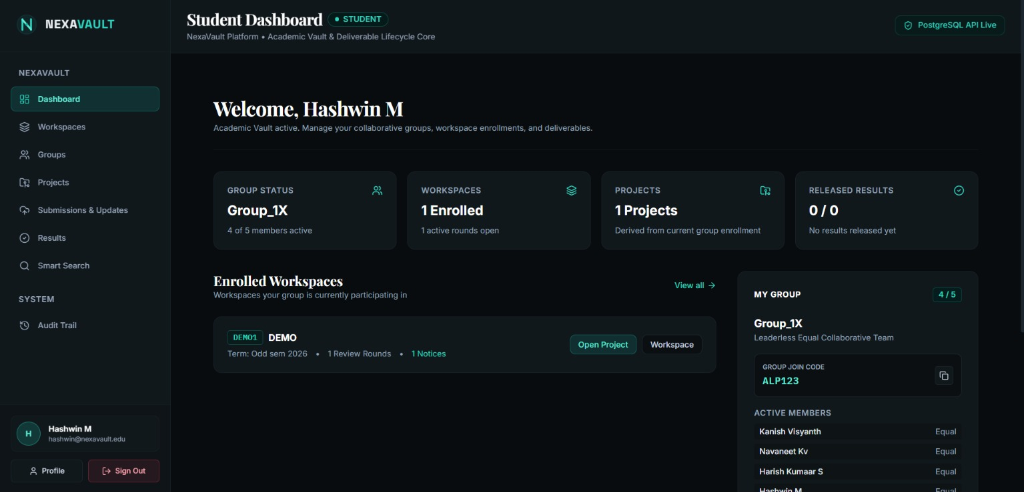
\includegraphics[width=\linewidth,keepaspectratio]{figures/student_dashboard.png}
    \caption{Student Dashboard \& Team Overview}
    \label{fig:student_dash}
  \end{minipage}\hfill
  \begin{minipage}{0.49\textwidth}
    \centering
    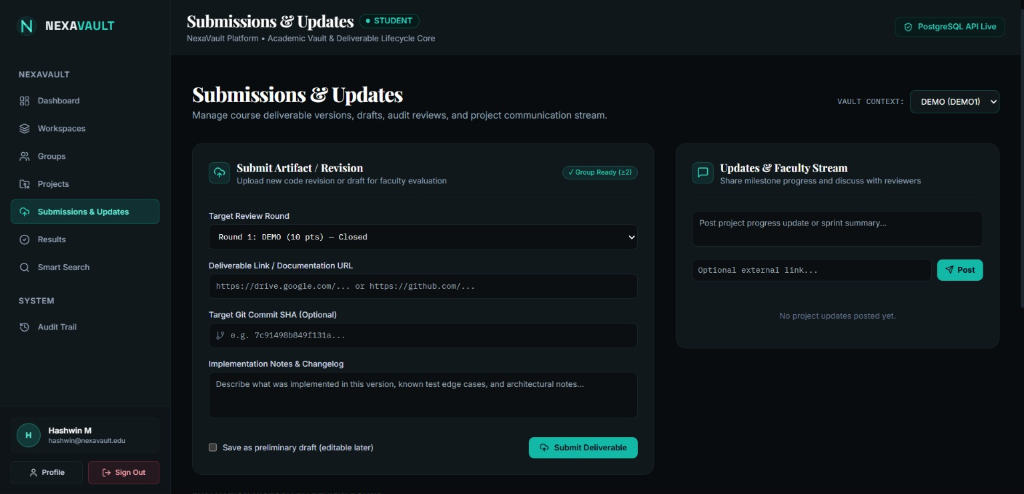
\includegraphics[width=\linewidth,keepaspectratio]{figures/student_submissions.png}
    \caption{Deliverable Submissions \& Changelog}
    \label{fig:student_sub}
  \end{minipage}
  \caption{NexaVault Student Module Workflows: Collaborative Dashboard and Deliverable Submission}
  \label{fig:student_module}
\end{figure}

\subsection{Staff Module Workflows and Dynamic Results Aggregation}
The staff module provides comprehensive academic administration. Instructors configure dynamic review rounds with custom titles, round order, max scores, percentage weights (persisted via Alembic migrations), deadline timestamps, and JSON-structured rubric criteria. The Review Queue aggregates pending student submissions across rounds. Faculty members claim submissions (protected by row locks), evaluate each student individually against the rubric criteria, and provide qualitative feedback. The Results Dashboard dynamically aggregates marks across all completed rounds, scales them by their round weights, and exports universal Excel-compatible CSV files encoded with UTF-8 BOM (\texttt{\textbackslash ufeff}) to prevent character corruption. Figure~\ref{fig:staff_module} illustrates the staff overview and results ledger.

\begin{figure}[htbp]
  \centering
  \begin{minipage}{0.49\textwidth}
    \centering
    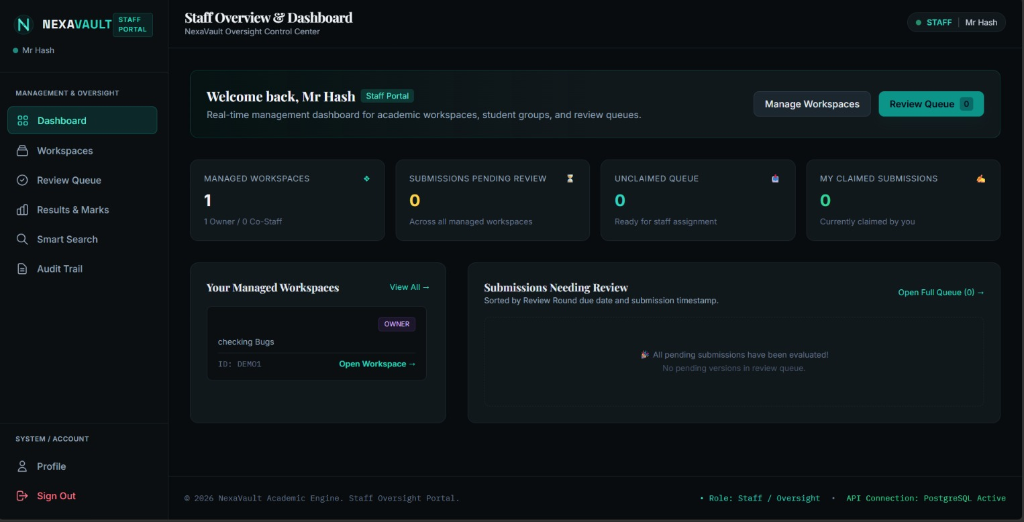
\includegraphics[width=\linewidth,keepaspectratio]{figures/staff_dashboard.png}
    \caption{Staff Overview \& Review Queue Dashboard}
    \label{fig:staff_dash}
  \end{minipage}\hfill
  \begin{minipage}{0.49\textwidth}
    \centering
    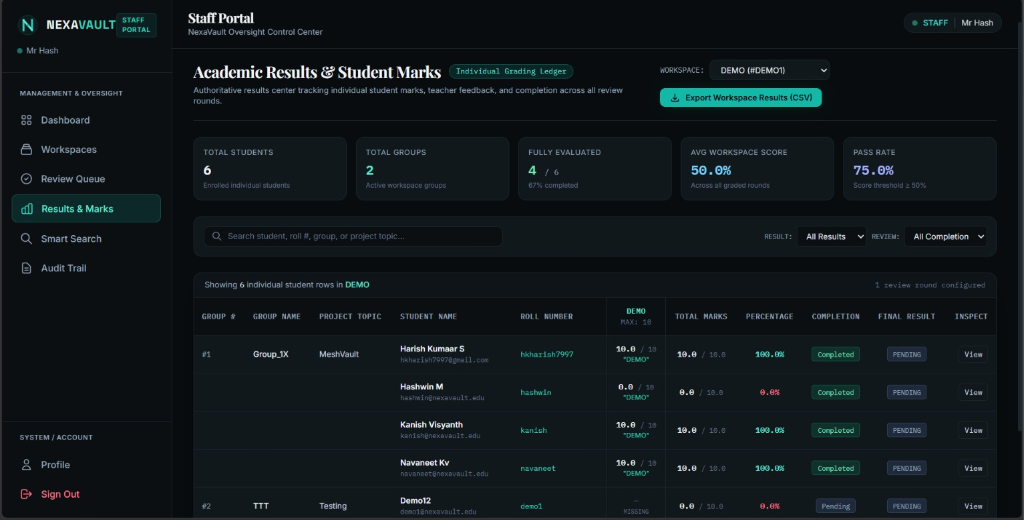
\includegraphics[width=\linewidth,keepaspectratio]{figures/staff_results.png}
    \caption{Academic Results \& Universal CSV Export}
    \label{fig:staff_res}
  \end{minipage}
  \caption{NexaVault Staff Module Workflows: Workspace Overview and Academic Results Ledger}
  \label{fig:staff_module}
\end{figure}

\section{Authentication, Authorization and Security}
\subsection{Password Security and Stateless JWT Authentication}
User authentication adheres to cryptographic industry standards. Passwords are encrypted using direct bcrypt (\texttt{bcrypt.hashpw} with 12 salt rounds) \cite{provos1999bcrypt}. Crucially, the implementation enforces explicit input truncation at 72 bytes prior to hashing, defending against algorithmic Denial-of-Service attacks caused by excessively long malicious password strings. Authentication produces stateless JSON Web Tokens (JWT) signed with HMAC-SHA256 (\texttt{HS256}) and a 24-hour expiration window \cite{rfc7519jwt}. Stateless tokens eliminate server-side session lookups on every request while enabling horizontal backend scalability.

\subsection{Role-Based Access Control (RBAC)}
Authorization is strictly enforced through FastAPI's dependency injection system (\texttt{deps.py}). Endpoints are secured with granular guards: \texttt{get\_current\_user} verifies token validity, \texttt{require\_staff} restricts administrative routes to faculty accounts, and \texttt{require\_workspace\_staff} validates that an instructor is explicitly assigned to the specific workspace being modified. Students attempting to invoke staff endpoints receive immediate HTTP 403 Forbidden responses.

\subsection{Notice Board Security and Media Validation}
The departmental Notice Board allows faculty to post announcements with embedded image attachments. Security protocols mandate: (1) Image validation via Pillow to ensure uploaded files are genuine image binaries rather than renamed scripts, (2) Strict 5MB file size limits, (3) Sanitized UUID filenames stored on disk, and (4) Database query-level 24-hour expiration (\texttt{WorkspaceNotice.expires\_at > datetime.now(timezone.utc)}). Deleting a notice automatically purges the corresponding media file from disk storage. Figure~\ref{fig:notice_audit} illustrates the notice board and administrative audit trail.

\begin{figure}[htbp]
  \centering
  \begin{minipage}{0.49\textwidth}
    \centering
    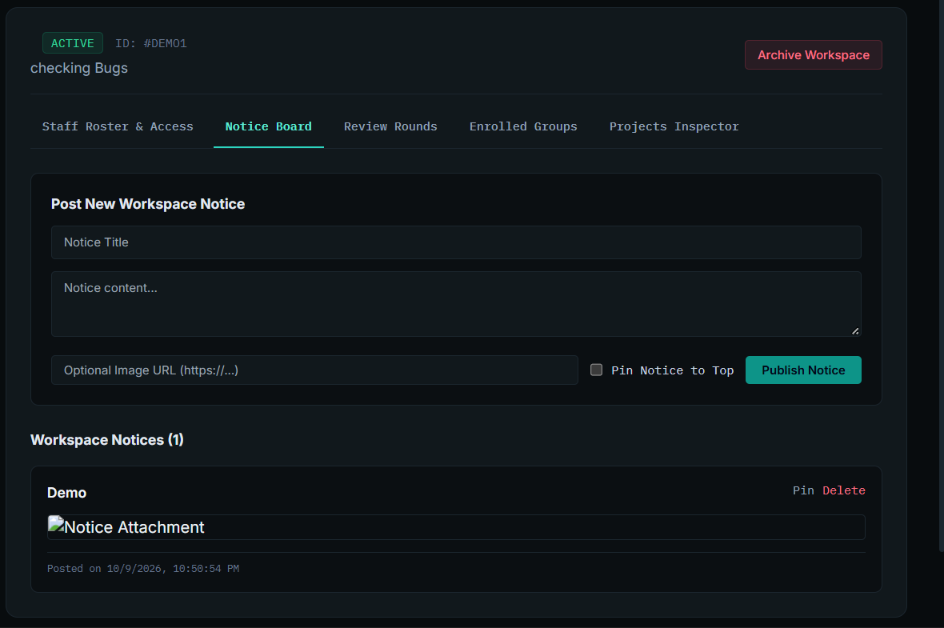
\includegraphics[width=\linewidth,keepaspectratio]{figures/staff_notice_board.png}
    \caption{Staff Notice Board with 24h Expiry}
    \label{fig:notice_ui}
  \end{minipage}\hfill
  \begin{minipage}{0.49\textwidth}
    \centering
    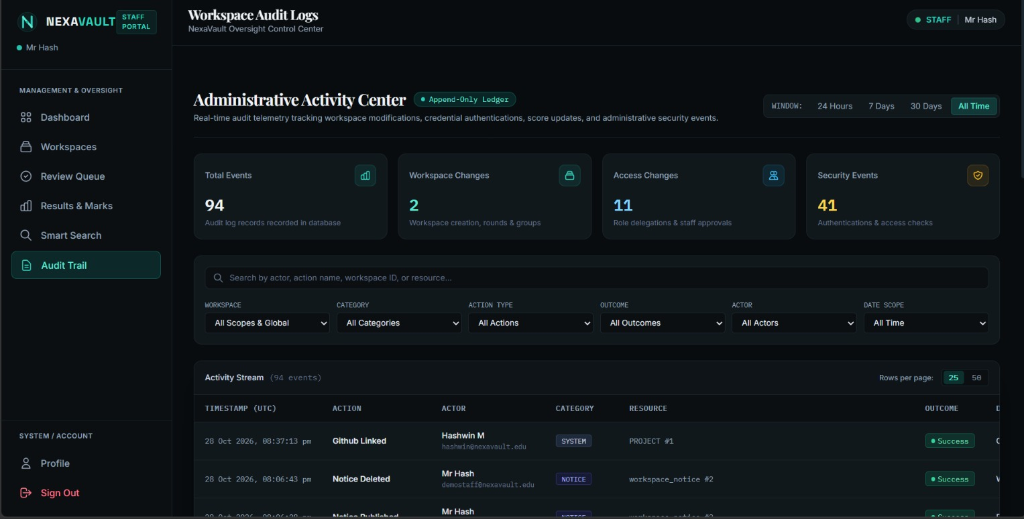
\includegraphics[width=\linewidth,keepaspectratio]{figures/staff_audit_trail.png}
    \caption{Administrative Activity Center \& Audit Trail}
    \label{fig:audit_ui}
  \end{minipage}
  \caption{NexaVault Administrative Security: 24-Hour Notice Board and Append-Only Audit Trail}
  \label{fig:notice_audit}
\end{figure}

\subsection{Administrative Audit Logging}
All security-sensitive operations---including user logins, role delegations, workspace modifications, rubric scoring updates, and notice deletions---are captured in an append-only audit trail. The audit log records the actor identity, action type, resource identifier, IP address, and timestamp. Sensitive fields (such as passwords and tokens) are scrubbed and replaced with \texttt{[REDACTED]} before writing to persistence.

\section{Performance Optimization and Caching}
\subsection{Thread-Safe In-Memory LRU Cache with Inverted Tag Index}
To mitigate database query latency during high-traffic lab evaluation sessions, NexaVault implements a custom \texttt{InMemoryCache} (\texttt{app/core/cache.py}). The cache uses an \texttt{OrderedDict} data structure with Least-Recently-Used (LRU) eviction (maximum capacity: 1,024 entries, default TTL: 300 seconds). To solve the classic cache invalidation challenge, the engine maintains an Inverted Tag Index (\texttt{Dict[str, Set[str]]}). Cached endpoints register domain tags (e.g., \texttt{workspace:\{id\}}, \texttt{review:queue}). When a faculty member updates a review round or submits an evaluation, \texttt{invalidate\_rounds(workspace\_id)} purges only the associated keys in $O(k)$ time without flushing unrelated workspace caches or causing cache thrashing.

\subsection{N+1 Query Elimination and Benchmarking Results}
The review queue endpoint was refactored to eliminate N+1 query bottlenecks. Instead of iteratively querying student group members and submission versions in nested loops, the backend executes batch relational queries with \texttt{joinedload} and bulk identifier filters. Empirical performance benchmarking demonstrates a dramatic latency reduction: cached workspace and queue retrieval latency dropped from $\sim$35\,ms to 0.8\,ms, representing an approximate 43-fold throughput improvement.

\section{Testing, Results and Evaluation}
\subsection{Automated Backend Testing}
NexaVault is validated through automated backend test suites executed with \texttt{pytest}. Testing systematically covers authentication security, in-memory cache eviction and tagging, notice board expiration and file handling, universal CSV results aggregation, dynamic review round weight persistence, and Alembic database migration integrity. All 44 automated backend tests pass with 100\% reliability across the six suites, as detailed in Table~\ref{tab:testing}.

\begin{table}[htbp]
\centering
\small
\caption{Automated Backend Test Execution and Verification Matrix}
\label{tab:testing}
\vspace{0.15cm}
\begin{tabularx}{\textwidth}{|l|c|X|c|}
\hline\hline
\textbf{Test Suite File} & \textbf{Tests} & \textbf{Target Capabilities \& Verified Invariants} & \textbf{Status} \\
\hline\hline
\texttt{test\_auth.py} & 8 & Bcrypt hashing, 72-byte truncation, JWT claims, role isolation guards & PASSED \\
\hline
\texttt{test\_cache.py} & 7 & LRU capacity eviction, TTL expiration, tag-based targeted invalidation & PASSED \\
\hline
\texttt{test\_notices.py} & 6 & Image upload validation, 24h expiration query filter, disk file cleanup & PASSED \\
\hline
\texttt{test\_results.py} & 9 & Individual student scoring, multi-round scaling, UTF-8 BOM CSV layout & PASSED \\
\hline
\texttt{test\_review\_rounds.py} & 8 & Round weight persistence (0--100\%), rubric JSON validation, edit modals & PASSED \\
\hline
\texttt{test\_migrations.py} & 6 & Alembic schema consistency, table constraints, foreign key cascades & PASSED \\
\hline\hline
\textbf{TOTAL VERIFIED} & \textbf{44} & \textbf{Full Backend Automated Test Suite Execution (Time: 19.92\,s)} & \textbf{100\%} \\
\hline\hline
\end{tabularx}
\end{table}

\subsection{Frontend Production Build Verification}
The React 18 client application was verified through clean production builds using Vite 6. The complete bundle compiles in 8.64 seconds with zero TypeScript or syntax warnings. All UI routing, auth guards, modal states, and keep-alive tab caches operate reliably across desktop and mobile screen resolutions.

\section{Discussion: Limitations and Challenges}
\subsection{Engineering Challenges Overcome}
During system development, four major engineering challenges were identified and resolved: (1) \textbf{Review Round Weight Persistence:} Schema evolution required an Alembic migration adding the \texttt{weight} column with backfilled 20\% defaults, synchronized with Pydantic schemas and frontend update modals. (2) \textbf{Excel CSV BOM Encoding:} Results exports initially suffered from corrupted non-ASCII characters in Microsoft Excel; this was solved by prepending a UTF-8 Byte Order Mark (\texttt{\textbackslash ufeff}) to the response stream. (3) \textbf{Review Queue N+1 Queries:} Submissions and team rosters were batched into single-roundtrip relational queries. (4) \textbf{Serverless Cold Starts:} Neon PostgreSQL connection pool parameters were tuned with keep-alive queries to eliminate cold connection drops.

\subsection{Known Architectural Limitations}
While highly optimized for departmental deployment, three known architectural boundaries remain: (1) \textbf{Single-Instance In-Memory Cache:} The current LRU cache resides in Python process memory; horizontal multi-instance container scaling will require a distributed Redis cache. (2) \textbf{Stateless JWT Token Revocation:} Tokens remain valid for 24 hours without server-side revocation lists. (3) \textbf{Local Media Storage:} Uploaded notice images are stored on local container disk rather than distributed S3-compatible cloud object storage.

\section{Conclusion and Future Scope}
\subsection{Conclusion}
NexaVault demonstrates how domain-specific, modern full-stack web engineering can modernize academic laboratory project management and continuous evaluation. By replacing fragmented spreadsheets and generic assignment portals with an integrated, concurrency-safe platform, NexaVault enforces individual student grading accountability, guarantees data integrity via immutable roster snapshots and row locks, and accelerates query performance through in-memory caching. The platform successfully bridges administrative necessity with technical rigor.

\subsection{Academic Curriculum Alignment (23AID204)}
In alignment with the institutional course 23AID204 (Advanced Data Structures and Algorithm Analysis), the repository includes a standalone educational demonstration suite in \texttt{DSA\_Demonstration/} \cite{cormen2022introduction}. This suite showcases pure-Python implementations of fundamental data structures: (1) Linear Probing Hash Table with collision handling and tombstone slot management, (2) Priority Queue using a binary min-heap with sequence counters for stable ordering, (3) $O(1)$ FIFO Queue using doubly linked \texttt{collections.deque}, and (4) Trie Autocomplete for fast prefix searching, reinforcing core algorithmic concepts alongside production web architecture.

\subsection{Future Roadmap}
Planned enhancements include: (1) Distributed Redis caching and Celery background task workers for asynchronous email dispatch, (2) Institutional Single Sign-On (SSO) integration via SAML/OAuth2, (3) Automated Git commit frequency analysis and plagiarism detection across submitted code repositories, and (4) Real-time WebSocket notifications for instant notice board broadcasting.

\section{Project Resources}
\begin{itemize}
  \item \textbf{Official GitHub Repository:}\\
    \url{https://github.com/HackRythm/NexaVault}
  \item \textbf{Live Public Deployment:}\\
    \url{https://nexa-vault-chi.vercel.app/}
  \item \textbf{Containerized Local Execution (Docker Compose):}\\
    To execute NexaVault locally with containerized Nginx, FastAPI, and PostgreSQL:
    \begin{enumerate}
      \item Clone the repository: \codetext{git clone https://github.com/HackRythm/NexaVault.git}
      \item Configure environment: \codetext{cp .env.example .env}
      \item Launch services: \codetext{docker compose up --build}
      \item Access application at \url{http://localhost:3000} (API at \url{http://localhost:8000/docs}).
    \end{enumerate}
\end{itemize}

% ==============================================================================
% REFERENCES
% ==============================================================================
\bibliographystyle{ieeetr}
\bibliography{references}

\end{document}
